\scanpage{70}
que dans le cas des cartes ordinaires, les relations intéressantes à considérer sont du type (30), à l'exclusion de $\unsure{(*)}$. \figure{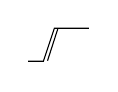
\begin{tikzpicture}[baseline=-.2ex,scale=.35]
\draw (0,0)--(.55,0)--(.95,1.2)--(2.2,1.2);
\draw (.7,.02)--(1.08,1.2);
\end{tikzpicture}} On considère que l'on a \deleted{\unsure{les arêtes}}\inserted{$\rho_i^\infty=1$} par définition, de sorte que l'on peut considérer un système de conditions (29), où pour tt $i\in\{0,1,\infty\}$, on a
\[
\text{(31)}\qquad \nu_i\in\overline{\mathbb N}^{*}=\mathbb N^{*}\cup\{+\infty\}.
\]

Les cartes (finies) pondérées triangulées correspondantes sont déterminées à l'aide du groupe quotient
\[
\text{(32)}\qquad
\Pi_{0,3}/\langle\rho_0^{\nu_0},\rho_1^{\nu_1},\rho_\infty^{\nu_\infty}\rangle
\qquad\text{(cas orienté)}
\]
ou par le quotient
\[
\text{(32 bis)}\qquad
\Pi_{0,3}^{\tau}/\langle\rho_0^{\nu_0},\rho_1^{\nu_1},\rho_\infty^{\nu_\infty}\rangle
\qquad\text{(cas non orienté)}
\]
qui s'identifie à une extension de $\{1,\tau\}$ par (32). Ce dernier groupe s'interprète comme groupe fondamental ``avec signature''
\[
\text{(33)}\qquad
\Pi_{0,3}/\langle(\rho_i^{\nu_i})\rangle
\simeq\Pi_1(\mathbb P^1(\mathbb C),\nu_*;P_+)
\]
\[
\nu_*=(\nu_0\unsure{R_0|P_0}+\nu_1\unsure{R_1|P_1}+\nu_\infty\unsure{R_\infty|P_\infty})
\quad\text{signature sur }\mathbb P^1_{\mathbb C}
\]
ou encore comme groupe fondamental de la multiplicité (topologique, analytique ou schématique, au choix -- mais dans ce dernier cas il s'agit du complété profini...)
\margin{69}
